\documentclass[twocolumn,superscriptaddress,showpacs,preprintnumbers,amsmath,amssymb,prl]{revtex4-1}
\usepackage{siunitx}
\usepackage{tikz}
\usetikzlibrary{arrows,shapes,backgrounds, calc, positioning, topaths,chains, intersections, decorations.markings, shapes.geometric, matrix,patterns,mindmap,fit}
%\usetikzlibrary{positioning, patterns,topaths,chains,matrix}

\usepackage{pgfplots}
\usepackage{pgfplotstable}
\pgfplotsset{compat=1.9}
\usepgfplotslibrary{groupplots}
\usepgfplotslibrary{external}
\tikzsetexternalprefix{fig_long/}
\tikzexternalize
\tikzset{external/force remake}

\begin{document}
\pgfplotscreateplotcyclelist{earthy}{%
red!40!black,
red!60!black,
red!80!black,
red,
red!80!yellow,
red!60!yellow,
red!40!yellow,
}
\tikzsetnextfilename{structure_confocal}
\begin{figure*}
\begin{tikzpicture}[every axis/.style={xlabel absolute, every axis x label/.append style={anchor=base, yshift=-1em}}]
\begin{groupplot}[
	group style={
			group name=g, group size=1 by 3,
			vertical sep=0.5em,
			xticklabels at=edge bottom,
		},
	height=7.5\baselineskip,
	width=0.3\textwidth,
	xmin=0, xmax=17, ymin=0,
	cycle list name=linestyles,
	no marks,
	]
\nextgroupplot[ylabel={$\xi$ (\si{\micro\metre})}]
\addplot table[skip coords between index={0}{64}, x expr={\thisrowno{0}/3600}]{ech17_pore_size.txt};
\addplot table[skip coords between index={0}{15}, x expr={\thisrowno{0}/3600}]{ech19_pore_size.txt};
\nextgroupplot[ylabel={$\chi$ (a.u.)}]
\begin{scope}[every node/.style={anchor=base west, font=\scriptsize}]
\addplot table[skip coords between index={0}{64}, x expr={\thisrowno{0}/3600}, y expr={\thisrowno{2}/1e7}]{ech17_pore_size.txt} node (l1) {1\%};
\addplot table[skip coords between index={0}{15}, x expr={\thisrowno{0}/3600}, y expr={\thisrowno{2}/1e7}]{ech19_pore_size.txt} node at ($(l1.base west)-(axis cs:0,1.8)$) {4\%};
\end{scope}
\nextgroupplot[xlabel={time (\si{\hour})}, ylabel={$\gamma$}]
\addplot table[skip coords between index={0}{64}, x expr={\thisrowno{0}/3600}, y index=3]{ech17_pore_size.txt};
\addplot table[skip coords between index={0}{15}, x expr={\thisrowno{0}/3600}, y index=3]{ech19_pore_size.txt};
\end{groupplot}


\matrix[matrix of nodes, inner sep=0, row sep=0.2em, column sep=0.2em, matrix anchor=north west] 
at ($(g c1r1.right of north east)+(-\textwidth,0)$)
(m) {
\SI{5}{\minute} & \SI{27}{\minute} & \SI{49}{\minute} & \SI{8}{\hour}\\
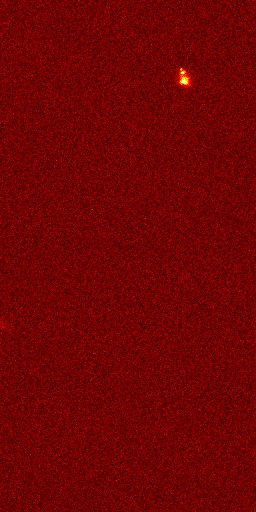
\includegraphics[width=5\baselineskip]{ech19_t001.jpg}&
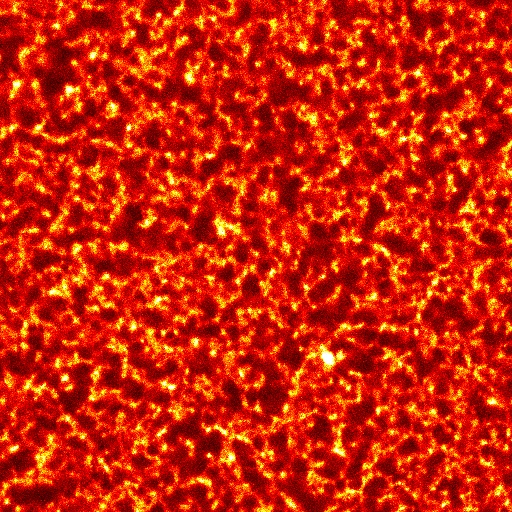
\includegraphics[width=5\baselineskip]{ech19_t043.jpg}&
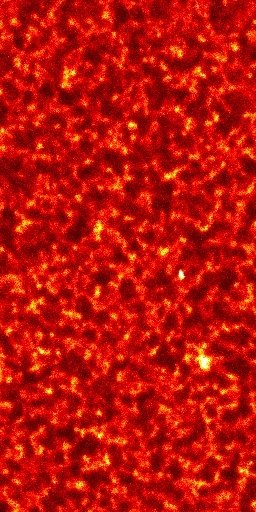
\includegraphics[width=5\baselineskip]{ech19_t085.jpg}&
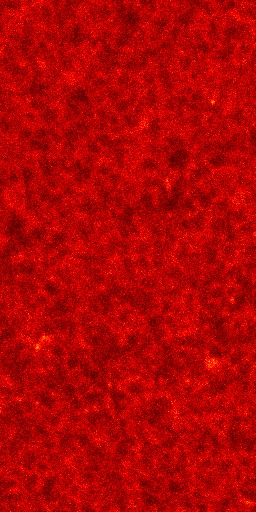
\includegraphics[width=5\baselineskip]{ech19_t132.jpg}\\
};
\draw[ultra thick, white] (m-2-1.south east) ++(-0.5\baselineskip,1em) -- +(-4\baselineskip,0);

\newdimen\mydima
\newdimen\mydimb
\pgfextracty{\mydima}{\pgfpointanchor{g c1r1}{north}}
\pgfextracty{\mydimb}{\pgfpointanchor{g c1r3}{south}}
\begin{loglogaxis}[
	name=Sq,
	scale only axis,
	width=0.24\textwidth,
	height=\mydima-\mydimb,
	anchor=left of north west,
	at={(m.north east)},
	cycle list name=earthy,
	xlabel={$q$ (\si{\per\micro\metre})},
	ylabel={$S(q)$ (a.u.)},
	domain=0.1:6.1,
	xmin=0.03, xmax=1e3,
	ymin=1e5,
	clip mode=individual,
	]
\begin{scope}[
	every axis plot post/.append style={only marks, mark options={scale=0.3}},
]
\addplot table{ech19_t016.Sq};
\addplot table{ech19_t018.Sq};
\addplot table{ech19_t020.Sq};
\addplot table{ech19_t022.Sq};
\addplot table{ech19_t024.Sq};
\addplot table{ech19_t026.Sq};
\addplot table{ech19_t028.Sq};

\pgfplotsset{cycle list shift=-7}
\addplot table[x expr={100*\thisrowno{0}}]{ech19_t049.Sq};
\addplot table[x expr={100*\thisrowno{0}}]{ech19_t091.Sq};
\addplot table[x expr={100*\thisrowno{0}}]{ech19_t095.Sq};
\addplot table[x expr={100*\thisrowno{0}}]{ech19_t110.Sq};
\addplot table[x expr={100*\thisrowno{0}}]{ech19_t132.Sq};
%\pgfplotsset{cycle list shift=2}
\addplot table[x expr={100*\thisrowno{0}}]{ech19_t183.Sq};
\end{scope}

\addplot[black,domain=0.1:2.3,] {1.41162e+06/(1+(0.863106*x)^(2.48957)} coordinate[pos=0] (t0);
% \addplot {3.08321e+06/(1+(0.675481*x)^(3.21053)};
% \addplot {7.21904e+06/(1+(0.682678*x)^(3.35995)};
% \addplot {1.2921e+07/(1+(0.682867*x)^(3.43546)};
% \addplot {2.00283e+07/(1+(0.679492*x)^(3.55078)};
% \addplot {2.65481e+07/(1+(0.672847*x)^(3.65046)};
\addplot[black] {3.10648e+07/(1+(0.674804*x)^(3.69175)} coordinate[pos=0] (t1);

\addplot[black,domain=10:610] {3.81303e+07/(1+(0.00643513*x)^(3.91326)} coordinate[pos=0] (t2);
% \addplot {2.28285e+07/(1+(0.00584224*x)^(3.83587)};
% \addplot {1.43395e+07/(1+(0.00654421*x)^(3.73896)};
% \addplot {9.58685e+06/(1+(0.00865948*x)^(2.84983)};
% \addplot {6.8931e+06/(1+(0.00946977*x)^(2.56298)};
\addplot[black,domain=10:373] {5.5388e+06/(1+(0.00950251*x)^(2.52804)} coordinate[pos=0] (t3);
\draw[->, ultra thick] (t0) -- (t1) node[midway,rotate=90, above, font=\footnotesize] {time};
\draw[->, ultra thick] (t2) -- (t3) node[midway,rotate=90, above, font=\footnotesize] {time};
\end{loglogaxis}
\begin{scope}[every node/.style={anchor=north west, text height=0.8em, text depth=0.2em}]
\node[white] at (m-2-1.north west) {(a)};
\node at (Sq.north west) {(b)};
\node[anchor=east] at (g c1r1.east) {(c)};
\node[anchor=east] at (g c1r2.east) {(d)};
\node[anchor=south east] at (g c1r3.south east) {(e)};
\end{scope}
\end{tikzpicture}
\end{figure*}

\tikzsetnextfilename{structure_finale}
%\begin{figure}
\begin{tikzpicture}[every node/.style={inner sep=0}]
\matrix[matrix of nodes, row sep=3pt, column sep=0] (m){
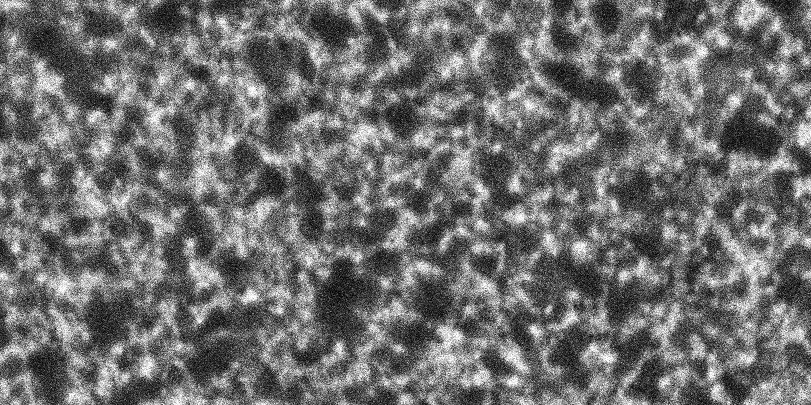
\includegraphics[width=\columnwidth]{ech17_x63_time699_crop.jpg}\\
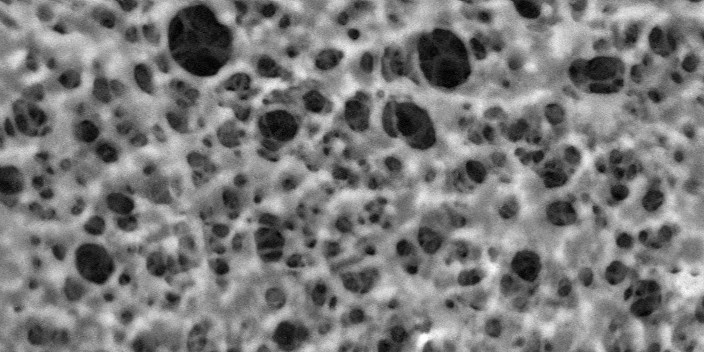
\includegraphics[width=\columnwidth]{ESEM_cas4_GDL1-17_crop.jpg}\\
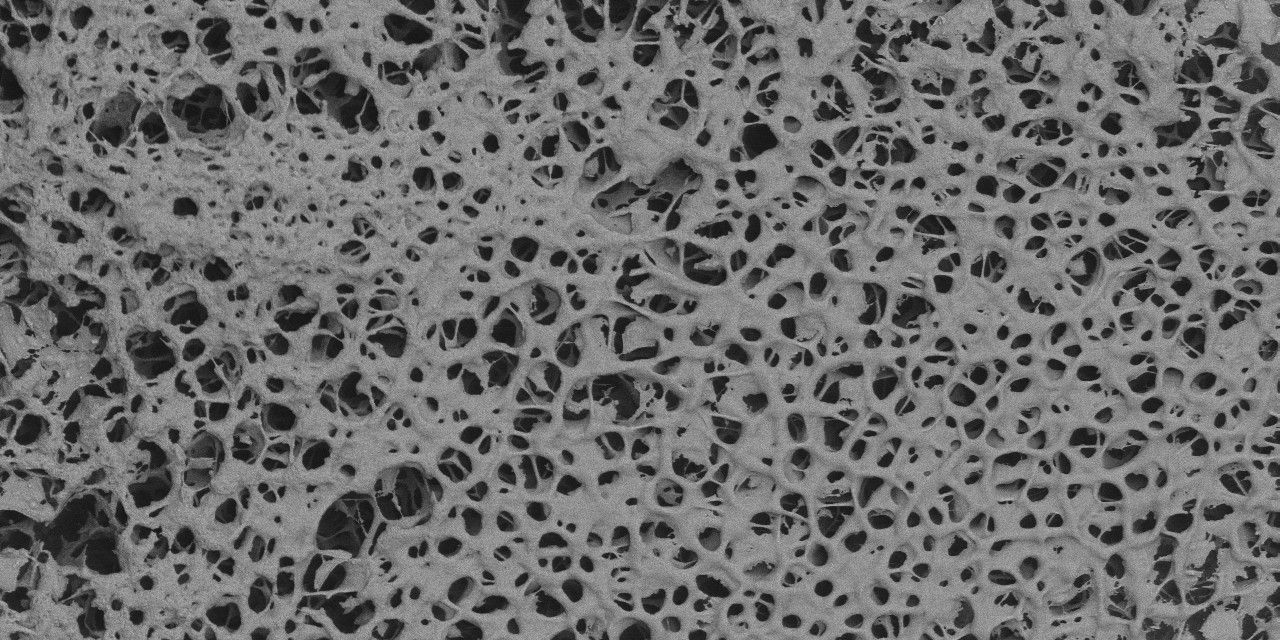
\includegraphics[width=\columnwidth]{SEM_cas4_gdl1_22_crop.jpg}\\
};
\foreach \i in {1,2,3}
\draw[ultra thick, white] (m-\i-1.south east) ++(-1em,1em) -- +(-0.25\columnwidth,0);
\end{tikzpicture}
\caption{Final structure of caseinate 4\%, GDL 4\% gels, observed by fluorescent confocal micoscopy, environmental SEM and cryo SEM.}
\end{figure}
\tikzsetnextfilename{prise_cas4}
%\begin{figure}
\begin{tikzpicture}
\begin{axis}[
	name=unscaled,
	height=0.5\columnwidth,
	width=\columnwidth-1em,
	xlabel={time (h)}, ylabel={$G^\prime$ (\si{\pascal})},
	cycle list name=earthy,
	no marks,
	xmin=0, xmax=20,ymin=0,
	]
	\begin{scope}[every node/.style={anchor=base west, inner xsep=0,font=\footnotesize}]
	\addplot table[x expr={\thisrowno{0}/3600}]{cas4_GDL1_Y265.prise} node {1\%};
	\addplot table[x expr={\thisrowno{0}/3600}]{cas4_GDL1.25_Y277.prise} node {1.25\%};
	\addplot table[x expr={\thisrowno{0}/3600}]{cas4_GDL1.5_Y275.prise} node {1.5\%};
	\addplot table[x expr={\thisrowno{0}/3600}]{cas4_GDL2_Y268.prise} node[yshift=0.1em] {2\%};
	\addplot table[x expr={\thisrowno{0}/3600}]{cas4_GDL3_Y270.prise} node[yshift=-0.1em] {3\%};
	\addplot table[x expr={\thisrowno{0}/3600}]{cas4_GDL4_Y271.prise} node[yshift=-0.6em] {4\%};
	\end{scope}
\end{axis}
\begin{loglogaxis}[
	name=scaled,
	anchor=north west, 
	at=(unscaled.below south west), 
	width=0.5\columnwidth-0.5em,
	height=0.375\columnwidth,
	cycle list name=earthy,
	no marks,
	xmin=1e-3, xmax=1e2, ymin=1e-3, ymax=2,
	xlabel=$(t-t_i)/(t_m-t_i)$, 
	ylabel=$G^\prime/G^\prime_m$ ,
]
	\addplot table[x expr={(\thisrowno{0}-7758)/(28840-7758)}, y expr={\thisrowno{1}/883}]{cas4_GDL1_Y265.prise};
	\addplot table[x expr={(\thisrowno{0}-5179)/(14240-5179)}, y expr={\thisrowno{1}/788}]{cas4_GDL1.25_Y277.prise};
	\addplot table[x expr={(\thisrowno{0}-3839)/(9640-3839)}, y expr={\thisrowno{1}/726}]{cas4_GDL1.5_Y275.prise};
	\addplot table[x expr={(\thisrowno{0}-2519)/(5720-2519)}, y expr={\thisrowno{1}/665}]{cas4_GDL2_Y268.prise};
	\addplot table[x expr={(\thisrowno{0}-1369)/(3120-1369)}, y expr={\thisrowno{1}/589}]{cas4_GDL3_Y270.prise};
	\addplot table[x expr={(\thisrowno{0}-758)/(1890-758)}, y expr={\thisrowno{1}/500}]{cas4_GDL4_Y271.prise};
\end{loglogaxis}
\begin{axis}[
	anchor=north east, 
	name=desc,
	at={(unscaled.below south east)}, 
	width=0.5\columnwidth-0.5em,
	height=0.375\columnwidth,
	cycle list name=earthy,
	no marks,
	xmode=log, xmin=1e-1, xmax=1e2,
	ymin=0, ymax=1.1,
	xlabel=$(t-t_m)/(t_m-t_i)$, 
	ylabel=$\displaystyle\frac{G^\prime-G^\prime_\infty}{G^\prime_m-G^\prime_\infty}$ ,
	%ylabel=$(G^\prime-G^\prime_\infty)/(G^\prime_m-G^\prime_\infty)$ ,
	]
	\addplot table[x expr={(\thisrowno{0}-28840)/(28840-7758)}, y expr={(\thisrowno{1}-616)/(883-616}]{cas4_GDL1_Y265.prise};
	\addplot table[x expr={(\thisrowno{0}-14240)/(14240-5179)}, y expr={(\thisrowno{1}-325)/(788-325}]{cas4_GDL1.25_Y277.prise};
	\addplot table[x expr={(\thisrowno{0}-9640)/(9640-3839)}, y expr={(\thisrowno{1}-200)/(726-200}]{cas4_GDL1.5_Y275.prise};
	\addplot table[x expr={(\thisrowno{0}-5720)/(5720-2519)}, y expr={(\thisrowno{1}-145)/(665-145}]{cas4_GDL2_Y268.prise};
	\addplot table[x expr={(\thisrowno{0}-3120)/(3120-1369)}, y expr={(\thisrowno{1}-103)/(589-103}]{cas4_GDL3_Y270.prise};
	\addplot table[x expr={(\thisrowno{0}-1890)/(1890-758)}, y expr={(\thisrowno{1}-75)/(500-75}]{cas4_GDL4_Y271.prise};
\end{axis}
\begin{scope}[every node/.style={anchor=south east, text height=0.8em, text depth=0.2em, font=\Large\bfseries}]
\node at (unscaled.south east) {a};
\node at (scaled.south east) {b};
\node at (desc.south east) {c};
\end{scope}
\end{tikzpicture}
\end{figure}
\tikzsetnextfilename{sweep_cas4}
%\begin{figure}
\begin{tikzpicture}
\pgfplotstableread{freqsweep_Y265_cas4_GDL1.txt}\GDLa
\pgfplotstableread{freqsweep_Y277_cas4_GDL1.25.txt}\GDLb
\pgfplotstableread{freqsweep_Y275_cas4_GDL1.5.txt}\GDLc
\pgfplotstableread{freqsweep_Y268_cas4_GDL2.txt}\GDLd
\pgfplotstableread{freqsweep_Y270_cas4_GDL3.txt}\GDLe
\pgfplotstableread{freqsweep_Y271_cas4_GDL4.txt}\GDLf

\begin{groupplot}[
	group style={
			group name=g, group size=1 by 2,
			vertical sep=0.5em,
			xticklabels at=edge bottom,
		},
	scale only axis,
	width=0.6\columnwidth-4em,
	height=0.3\columnwidth-2em,
	domain={6e-2:70},
	cycle list name=earthy,
	xmode=log, ymode=log,
	xmin=5e-2, xmax=1e3,
	xlabel absolute, every axis x label/.append style={anchor=base, yshift=-1em}
	]
\nextgroupplot[ylabel={$G^\prime$ (\si{\pascal})}]
\begin{scope}[
	every axis plot post/.append style={only marks, mark=*, mark options={scale=0.1}},
	every node/.style={anchor=west, ,font=\scriptsize, pos=0}
]
	\addplot table{\GDLa} node{1\%};
	\addplot table{\GDLb} node{1.25\%};
	\addplot table{\GDLc} node{1.5\%};
	\addplot table{\GDLd} node{2\%};
	\addplot table{\GDLe} node{3\%};
	\addplot table{\GDLf} node{4\%};
\end{scope}
\pgfplotsset{cycle list shift=-6}
\addplot {590.277*x^0.139256};
\addplot {349.762*x^0.121815};
\addplot {246.573*x^0.102707};
\addplot {162.851*x^0.0676911};
\addplot {109.351*x^0.0437222};
\addplot {76.7364*x^0.035779};



\nextgroupplot[ylabel={$G^{\prime\prime}$ (\si{\pascal})}, xlabel={$f$ (\si{\hertz})},]
\begin{scope}[
	every axis plot post/.append style={only marks, mark=*, mark options={scale=0.1}},
	every node/.style={anchor=west,font=\scriptsize, pos=0}
]
	\addplot table[y index=2]{\GDLa} node{1\%};
	\addplot table[y index=2]{\GDLb} node{1.25\%};
	\addplot table[y index=2]{\GDLc} node{1.5\%};
	\addplot table[y index=2]{\GDLd} node{2\%};
	\addplot table[y index=2]{\GDLe} node{3\%};
	\addplot table[y index=2]{\GDLf} node{4\%};
\end{scope}
\pgfplotsset{cycle list shift=-6}
\addplot {140.022*x^0.139256};
\addplot {72.4462*x^0.121815};
\addplot {43.0813*x^0.102707};
\addplot {18.9117*x^0.0676911};
\addplot {8.39838*x^0.0437222};
\addplot {4.99978*x^0.035779};
\end{groupplot}
\begin{axis}[
	name=alpha,
	anchor={left of south west},
	at={(g c1r2.right of south east)},
	scale only axis,
	width=0.4\columnwidth-4em-5pt,
	height=0.6\columnwidth-3.5em,
	xlabel={GDL (\%)},
	xmin=0, xmax=4.5,
	ylabel=$\alpha$, ymin=0,ymax=0.15,
	ytick={0,0.05,0.1}, yticklabels={0,0.05,0.10},
	xlabel absolute, every axis x label/.append style={anchor=base, yshift=-1em}
]
\addplot[mark=*] file{sweep_exponents.txt};
\end{axis}

\begin{scope}[every node/.style={anchor=north west, text height=0.8em, text depth=0.2em}]
\node at (g c1r1.north west) {(a)};
\node at (g c1r2.north west) {(b)};
\node[anchor=north east] at (alpha.north east) {(c)};
\end{scope}
\end{tikzpicture}
\end{figure}
\tikzsetnextfilename{prise_cas2_gdl05_T}
%\begin{figure}
\begin{tikzpicture}
\begin{axis}[
	name=main,
	scale only axis,
	width=\columnwidth-5em,
	cycle list name=earthy,
	xlabel={time (\si{\hour})},
	ylabel={$G^\prime$ (\si{\pascal})},
	xmin=0, xmax=20, ymin=0,
]
\begin{scope}[
	every node/.style={anchor=south east ,font=\scriptsize}
]
\addplot table[x expr=\thisrowno{0}/3600]{yaourt_2pc_0p5_T10.prise} node{\SI{10}{\degreeCelsius}};
\addplot table[x expr=\thisrowno{0}/3600]{yaourt_2pc_0p5_T15.prise} node{\SI{15}{\degreeCelsius}};
\addplot table[x expr=\thisrowno{0}/3600]{yaourt_2pc_0p5_T20.prise} node{\SI{20}{\degreeCelsius}};
\addplot table[x expr=\thisrowno{0}/3600]{yaourt_2pc_0p5_T25.prise} node{\SI{25}{\degreeCelsius}};
\addplot table[x expr=\thisrowno{0}/3600]{yaourt_2pc_0p5_T30.prise} node{\SI{30}{\degreeCelsius}};
\end{scope}
\end{axis}
\begin{axis}[
	anchor=below south east,
	at={($(main.south east)+(-0.5em,0)$)},
	small,
	scale only axis,
	width=0.4\columnwidth-4em,
	height=0.5\columnwidth-2em,
	xlabel={$300/T$ (\si{\per\kelvin})},
	ylabel={$G^\prime_\infty$ (\si{\pascal})},
	axis background/.style={fill=white}, 
	xtick={1,1.05},
	%xmode=log,
	%ymode=log,
]
\addplot[black, mark=*, only marks] table[x expr={300/(\thisrowno{0}}]{yaourt_2pc_0p5.Ginf};
\end{axis}
\end{tikzpicture}
\end{figure}
\tikzsetnextfilename{creep_cas4_gdl4}
%\begin{figure*}
\begin{tikzpicture}
\begin{groupplot}[
	group style={
			group name=g, group size=4 by 1,
			horizontal sep=4em,
			xticklabels at=edge bottom,
		},
	width=0.5\columnwidth,
%	height=0.3\columnwidth-2em,
	cycle list name=earthy,
	xmode=log, ymode=log,
	%xmin=5e-2, xmax=1e3,
	xlabel absolute, every axis x label/.append style={anchor=base, yshift=-1em},
	ylabel={$\dot{\gamma}/\dot{\gamma}_\text{min}$},
	extra tick style={grid=major},%
	]
\nextgroupplot[
	xlabel={$t$ (\si{\second})}, ylabel={$\gamma$}, 
	ymax=3, ymin=2e-1,xmin=0.3,xmax=1e6,
	ytick={0.1,0.2,0.4,0.8,1.6}, yticklabels={0.1,0.2,0.4,0.8,1.6},
	extra y ticks={1}, extra y tick labels={},]
%\begin{scope}[every node/.style={font=\scriptsize, anchor=north west, inner xsep=0}]
\addplot table {Y242_20Pa_gamma_decimated.txt};% node[pos=0.5, rotate=35] {\SI{20}{\pascal}};
\addplot table {Y239_40Pa_gamma_decimated.txt};% node[pos=0.4, rotate=35] {\SI{40}{\pascal}};
\addplot table {Y238_50Pa_gamma_decimated.txt};% node[anchor=south east, rotate=90] at (rel axis cs:0.78,1) {\SI{50}{\pascal}};
\addplot table {Y246_60Pa_gamma_decimated.txt};% node[anchor=south east, rotate=90] at (rel axis cs:0.6,1) {\SI{60}{\pascal}};
\addplot table {Y236_100Pa_gamma_decimated.txt};% node[pos=0.1, rotate=15] {\SI{100}{\pascal}};
\addplot+[restrict x to domain=0.05:100] table {Y249_120Pa_gamma_decimated.txt};% node[anchor=north east, rotate=80] at (rel axis cs:0.15,1) {\SI{120}{\pascal}};
%\end{scope}

\nextgroupplot[xlabel={$t/\tau_f$},xmin=1e-5, xmax=2, ymin=0.5, ymax=5e4]
\addplot table {Y242_20Pa_gdot_decimated.txt};
\addplot table {Y239_40Pa_gdot_decimated.txt};
\addplot table {Y238_50Pa_gdot_decimated.txt};
\addplot table {Y246_60Pa_gdot_decimated.txt};
\addplot table {Y236_100Pa_gdot_decimated.txt};
\addplot+[restrict x to domain=-2.75:1] table {Y249_120Pa_gdot_decimated.txt};

\nextgroupplot[
	xlabel={$t/\tau_f$}, xmode=linear, ymode=linear, 
	xmin=0, xmax=1,ymin=0.5,ymax=10, restrict y to domain=0:11,
	ytick={2,4,6,8}]
\addplot table {Y242_20Pa_gdot_decimated.txt};
\addplot table {Y239_40Pa_gdot_decimated.txt};
\addplot table {Y238_50Pa_gdot_decimated.txt};
\addplot table {Y246_60Pa_gdot_decimated.txt};
\addplot table {Y236_100Pa_gdot_decimated.txt};
\addplot table {Y249_120Pa_gdot_decimated.txt};

\nextgroupplot[xlabel={$1-t/\tau_f$},xmin=1e-5, xmax=2, x dir=reverse, ymin=0.5, ymax=5e4]
\addplot table[x expr={1-\thisrowno{0}}] {Y242_20Pa_gdot_decimated.txt};
\addplot table[x expr={1-\thisrowno{0}}] {Y239_40Pa_gdot_decimated.txt};
\addplot table[x expr={1-\thisrowno{0}}] {Y238_50Pa_gdot_decimated.txt};
\addplot table[x expr={1-\thisrowno{0}}] {Y246_60Pa_gdot_decimated.txt};
\addplot table[x expr={1-\thisrowno{0}}] {Y236_100Pa_gdot_decimated.txt};
\addplot table[x expr={1-\thisrowno{0}}] {Y249_120Pa_gdot_decimated.txt};
\end{groupplot}
\end{tikzpicture}
\end{figure*}
\tikzsetnextfilename{basquin}
%\begin{figure}
\begin{tikzpicture}[every axis/.style={xlabel absolute, every axis x label/.append style={anchor=base, yshift=-1em}, ylabel absolute, every axis y label/.append style={anchor=base, yshift=-1em}}]
\begin{groupplot}[
	group style={
			group name=g, group size=2 by 2,
		    horizontal sep=4em,
			vertical sep=3.5em,
%			xticklabels at=edge bottom,
			%y descriptions at=edge left,
		},
	scale only axis,
	width=0.5\columnwidth-4.25em,
	xmode=log, ymode =log,
	ymax=2e6, xmin=0.125, xmax=2,
	xlabel=$\sigma/G^\prime$,
	ylabel={$\tau_m$ (\si{\second})},
	cycle list name=earthy,
	clip mode=individual,
	%cycle list shift=2,
	%ymin=0.01, ymax=1e6,
%	xmin=0, xmax=17, ymin=0,
%	cycle list name=linestyles,
%	no marks,
	]

%composition
\nextgroupplot[xlabel={$\sigma$ (\si{\pascal})}, xmin=10, xmax=2e3, ymin=2e-2, ytickten={-1,1,3,5}]
%\pgfplotsset{cycle list shift=3}
\addplot+[only marks, mark=square*] table[y index=5]{MCR_cas4_GDL1_gap10.txt};
\addplot+[only marks, mark=square, black] table[y index=5]{MCR_cas4_GDL4_gap10.txt};
%fits
\addplot[gray, domain=150:1000] {3.7e17*x^(-5.5)};
\addplot[gray, domain=20:350] {3.7e12*x^(-5.5)};

%composition rescaled
\nextgroupplot[xmax=4, ymin=2e-2, xtick={0.25, 0.5, 1, 2,4}, xticklabels={0.25, 0.5, 1, 2,4}, ytickten={-1,1,3,5}]
\addplot+[only marks, mark=square*] table[x expr={\thisrowno{0}/\thisrowno{2}}, y index=5]{MCR_cas4_GDL1_gap10.txt};
\addplot+[only marks, mark=square, black] table[x expr={\thisrowno{0}/\thisrowno{2}}, y index=5]{MCR_cas4_GDL4_gap10.txt};
%fit
\addplot[gray, domain=0.18:3.5] {40.6*x^(-5.5)};

%gap
\nextgroupplot[xtick={0.25, 0.5, 1}, xticklabels={0.25, 0.5, 1}, ymin=8]
%\addplot+[only marks] table[x expr={\thisrowno{0}/\thisrowno{2}}, y index=5]{MCR_cas4_GDL1_gap05.txt};
%\pgfplotsset{cycle list shift=2}
\addplot+[only marks, mark=square*] table[x expr={\thisrowno{0}/\thisrowno{2}}, y index=5]{MCR_cas4_GDL1_gap10.txt};
\pgfplotsset{cycle list shift=3}
\addplot+[only marks, mark=diamond*] table[x expr={\thisrowno{0}/\thisrowno{2}}, y index=5]{MCR_cas4_GDL1_gap15.txt};
\addplot+[only marks, mark=*] table[x expr={\thisrowno{0}/\thisrowno{2}}, y index=5]{MCR_cas4_GDL1_gap30.txt};
%fit
\addplot[gray, domain=0.2:1.3] {40.6*x^(-5.5)};
\addplot[gray, domain=0.17:0.5] {0.77*x^(-5.5)};

%gap rescaled
\nextgroupplot[ylabel={$\tau_m e^3$ (\si{\cubic\milli\metre\second})},xtick={0.25, 0.5, 1}, xticklabels={0.25, 0.5, 1}, ymin=8]
%\addplot+[only marks] table[x expr={\thisrowno{0}/\thisrowno{2}}, y expr={\thisrowno{5}*0.5^3}]{MCR_cas4_GDL1_gap05.txt};
%\pgfplotsset{cycle list shift=2}
\addplot+[only marks, mark=square*] table[x expr={\thisrowno{0}/\thisrowno{2}}, y expr={\thisrowno{5}*1^3}]{MCR_cas4_GDL1_gap10.txt};
\pgfplotsset{cycle list shift=3}
\addplot+[only marks, mark=diamond*] table[x expr={\thisrowno{0}/\thisrowno{2}}, y expr={\thisrowno{5}*1.5^3}]{MCR_cas4_GDL1_gap15.txt};
\addplot+[only marks, mark=*] table[x expr={\thisrowno{0}/\thisrowno{2}}, y expr={\thisrowno{5}*3^3}]{MCR_cas4_GDL1_gap30.txt};
%fit
\addplot[gray, domain=0.15:1.3] {34.9*x^(-5.5)};


\end{groupplot}
\begin{scope}[every node/.style={anchor=north east, text height=0.8em, text depth=0.2em}]
\node at (g c1r1.north east) {(a)};
\node at (g c2r1.north east) {(b)};
\node at (g c1r2.north east) {(c)};
\node at (g c2r2.north east) {(d)};
\end{scope}
\end{tikzpicture}
\end{figure}
\tikzsetnextfilename{MonkmanGrant}
%\begin{figure}
\begin{tikzpicture}[every axis/.style={xlabel absolute, every axis x label/.append style={anchor=base, yshift=-1em}, ylabel absolute, every axis y label/.append style={anchor=base, yshift=-1em}}]
\begin{groupplot}[
	group style={
			group name=g, group size=1 by 2,
			vertical sep=0.5em,
%			xticklabels at=edge bottom,
			x descriptions at=edge bottom,
		},
	width=\columnwidth,
	height=15\baselineskip,
	xmode=log, xmin=1, xmax=1e6,
	xlabel={$\tau_f$ (\si{\second})},
	domain=1:1e6,
]

\nextgroupplot[ylabel={$\tau_m$ (\si{\second})}, ymode=log]
\addplot[only marks, mark=*] table[x index=4, y index=5]{MCR_cas4_GDL1_gap10.txt};
\addplot[only marks, mark=square*] table[x index=4, y index=5]{MCR_cas4_GDL1_gap30.txt};
\addplot[gray, only marks, mark=o] table[x index=4, y index=5]{ARG2_cas4_GDL1_gap20.txt};
\addplot[red, only marks, mark=star] table[x index=4, y index=5]{MCR_cas4_GDL4_gap10.txt};
\addplot[no marks]{0.6*x};
\addplot[no marks, dashed]{0.4*x};

\nextgroupplot[ylabel=$\tau_m/\tau_f$, ymin=0]
\addplot[only marks, mark=*] table[x index=4, y expr={\thisrowno{5}/\thisrowno{4}}]{MCR_cas4_GDL1_gap10.txt};
\addplot[only marks, mark=square*] table[x index=4, y expr={\thisrowno{5}/\thisrowno{4}}]{MCR_cas4_GDL1_gap30.txt};
\addplot[gray, only marks, mark=o] table[x index=4, y expr={\thisrowno{5}/\thisrowno{4}}]{ARG2_cas4_GDL1_gap20.txt};
\addplot[red, only marks, mark=star] table[x index=4, y expr={\thisrowno{5}/\thisrowno{4}}]{MCR_cas4_GDL4_gap10.txt};
\addplot[no marks]{0.6};
\addplot[no marks, dashed]{0.4};

\end{groupplot}
\begin{scope}[every node/.style={anchor=south east, text height=0.8em, text depth=0.2em}]
\node at (g c1r1.south east) {(a)};
\node at (g c1r2.south east) {(b)};
\end{scope}
\end{tikzpicture}
\end{figure}
\tikzsetnextfilename{lambda}
%\begin{figure}
\begin{tikzpicture}
\begin{groupplot}[
	group style={
			group name=g, group size=1 by 2,
			vertical sep=3.5em,
%			xticklabels at=edge bottom,
			%y descriptions at=edge left,
		},
	width=\columnwidth,
	height=10\baselineskip,
	xmin=0, ymin=0,
	ylabel={$\lambda$ (\si{\milli\metre})},
]

\nextgroupplot[xlabel={$\sigma$ (\si{\pascal})}, xmax=900]
\addplot[only marks, error bars/.cd, y dir=both, y explicit] table[y error=erreur]{lambda_sigma_cas4_GDL1_ARG2.txt};
\addplot[mark=o, only marks, error bars/.cd, y dir=both, y explicit] table[y error=erreur]{lambda_sigma_cas4_GDL4_ARG2.txt};
\addplot[no marks, domain=0:900] {2.61};
\addplot[no marks, dotted, domain=0:900] {3.25};

\nextgroupplot[xlabel={gap (\si{\milli\metre})}, xmax=3.5, cycle list name=earthy]
\addplot[mark=o, only marks, error bars/.cd, y dir=both, y explicit] table[x=gap, y=lambda, y error=erreur, restrict expr to domain={\thisrowno{0}}{20:26}]{lambda_gap_cas4GDL4.txt};
\addplot+[mark=*, only marks, error bars/.cd, y dir=both, y explicit] coordinates{(2,2.61) +- (0,0.34)};
\pgfplotsset{cycle list shift=2};
\addplot+[mark=diamond*, only marks, error bars/.cd, y dir=both, y explicit] table[x=gap, y=lambda, y error=erreur, restrict expr to domain={\thisrowno{0}}{30:38}]{lambda_gap_cas4GDL4.txt};
\pgfplotsset{cycle list shift=3};
\addplot+[mark=triangle*, only marks, error bars/.cd, y dir=both, y explicit] table[x=gap, y=lambda, y error=erreur, restrict expr to domain={\thisrowno{0}}{38:50}]{lambda_gap_cas4GDL4.txt};
\addplot[no marks, domain=0:4] {1.3*x};
%\addplot[only marks, error bars/.cd, y dir=both, y explicit] table[x=gap, y expr={\thisrow{lambda}}, y error=erreur]{lambda_gap_cas4GDL1.txt};

\end{groupplot}
\newdimen\mydima
\pgfextractx{\mydima}{\pgfpointanchor{g c1r1}{north east}}
\node[inner sep=0, above left =1em and 0 of g c1r1.north east] (im) {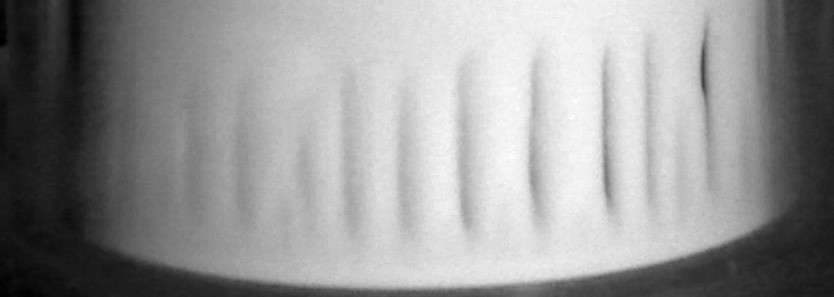
\includegraphics[width=\mydima]{Y140_bottom}};
\draw[<->] (im.north west) ++ (0.48\mydima, -0.2\mydima) -- +(0.075\mydima,0) node[midway,above] {$\lambda$};

\begin{scope}[every node/.style={anchor=south east, text height=0.8em, text depth=0.2em}]
\node[white] at (im.south east) {(a)};
\node at (g c1r1.south east) {(b)};
\node at (g c1r2.south east) {(c)};
\end{scope}
\end{tikzpicture}
\end{figure}
\end{document}